\section{Thorin type forms of the reciprocal zeta function}\label{ch:rz1}

Stieltjes inversion gives the Thorin type measure of a single Euler factor, a cosine series of both signs. The Lai and Vere-Jones identity replaces the exponentials of the Dirichlet series by hyperbolic secants, whose Thorin measures are lattices of unit atoms, at the price of M\"obius signs in the coefficients. Under RH the Thorin measure of the normalised reciprocal zeta function is $dM$, where $M-1$ is the argument function $S(\sqrt t)$. Its heat trace, the canonical function $w$ of Theorem~\ref{rz:thm:w}, is explicit in the primes, is an absolutely convergent series of Jacobi theta functions, and gives a criterion for RH (Theorem~\ref{rz:thm:crit}). Section~\ref{rz:sec:strip} follows these objects across the critical strip.

\subsection{The question and the three functions}\label{rz:sec:intro}

Write $\sqs$ for the principal square root on the cut plane $\cut$, so that $\Re\sqs>0$ there, and evaluate $\zeta$ at $z=\frac12+\sqs$. A zero $\rho=\frac12+i\gamma$ then corresponds to $\sqs=i\gamma$, that is to $s=-\gamma^2$, a point of the cut, and an atom of a Thorin measure at $t$ produces a singularity at $s=-t$, also on the cut. The Riemann Hypothesis therefore says that every zero sits where a Thorin atom could sit, which is the reason for the variable $\sqs$ here, as in Section~\ref{ch:clock}. The question of this chapter and of Chapter~\ref{chap:rzid} is whether the zeros, the primes and the gamma factor assemble into a Thorin measure, and if so which one. The two chapters have their own coordinates, which hold throughout both unless stated otherwise: $s$ is the variable $u$ of Sections~\ref{ch:clock} and \ref{ch:ggc}, $t$ is the variable $z$ of their Thorin measures, $x$ is the time of the heat trace $W(x)$, $\tau$ is the ordinate, and $z$ is the argument of $\zeta$ and $\xi$.

The M\"obius series and the Euler product converge absolutely to the right of the parabola $x=\frac14-y^2$, on
\[
H_{1/2}=\{s:\Re\sqs>\tfrac12\}=\{x+iy:\ x>\tfrac14-y^2\},
\]
and there
\begin{equation}\label{rz:eq:basic}
\frac{1}{\zeta(\frac12+\sqs)}=\sum_{n\ge1}\frac{\mu(n)}{\sqrt n}\,e^{-\sqs\log n}
=\prod_{p}\Bigl(1-p^{-1/2}e^{-\sqs\log p}\Bigr).
\end{equation}
Every term is built from $e^{-\lambda\sqs}$, which is completely monotone in $s$: it is the Laplace transform of the positive stable law of index $\frac12$, the law of the first passage time of $\sqrt2B$ to the level $\lambda$, where $B$ is a standard Brownian motion,
\begin{equation}\label{rz:eq:levy}
e^{-\lambda\sqs}=\int_0^\infty e^{-sx}\,\frac{\lambda}{2\sqrt\pi}\,x^{-3/2}e^{-\lambda^2/4x}\,dx .
\end{equation}
So \eqref{rz:eq:basic} writes $1/\zeta(\frac12+\sqs)$ as a signed series of Laplace transforms of stable laws. The Thorin measure, however, is read from the logarithm. Recall from \eqref{eq:ch3:ggc} that a generalised gamma convolution (GGC) has Laplace transform
\begin{equation}\label{rz:eq:thorin}
f(s)=\exp\Bigl(-as-\int_{(0,\infty)}\log\bigl(1+\tfrac st\bigr)\,U(dt)\Bigr),
\end{equation}
with $a\ge0$ and $U\ge0$ the Thorin measure; equivalently $-f'/f(s)=a+\int U(dt)/(s+t)$ is a Stieltjes function \cite{Bondesson}. We allow $U$ to be signed, with $\int_{(0,1)}|\log t|\,|U|(dt)+\int_{[1,\infty)}t^{-1}|U|(dt)<\infty$ so that the integral converges, and then call \eqref{rz:eq:thorin} a Thorin type representation.

Three functions of $s$ run through both chapters. The function $1/\zeta(\frac12+\sqs)$ vanishes at $s=\frac14$, where $\zeta$ has its pole, and equals $1/\zeta(\frac12)<0$ at $s=0$, so it is not the Laplace transform of a probability law. Both defects are removed by the normalised reciprocal zeta function
\begin{equation}\label{rz:eq:phi}
\varphi(s)=\frac{\zeta(\frac12)}{(1-4s)\,\zeta(\frac12+\sqs)},\qquad \varphi(0)=1 .
\end{equation}
The other two are the gamma factor $G(s)=\Gamma(\frac14+\frac\sqs2)\pi^{-\sqs/2}/\Gamma(\frac14)$ and the reciprocal Xi function $R(s)=\xi(\frac12)/\xi(\frac12+\sqs)$, and $\varphi=RG$ (Proposition~\ref{rz:prop:rh}). In both chapters $G$ is the gamma factor, not the function $G$ of Section~\ref{ch:clock}, whose reciprocal is $R$, except in Section~\ref{rz:sec:polya}, where $G$ is a Laguerre P\'olya function; and $\theta(\tau)=\Im\log\Gamma(\frac14+\frac{i\tau}{2})-\frac\tau2\log\pi$ is the Riemann Siegel theta function, written $\vartheta$ elsewhere in the book (Section~\ref{ch:classical}), so that $\theta'(\tau)=\frac12\Re\psi(\frac14+\frac{i\tau}2)-\frac12\log\pi$ \cite[Section 6.5]{Edwards}. Table~\ref{rz:tab:measures} lists the Thorin measures of the three functions and of the building blocks used below. In it $N(T)$ counts the zeros with $0<\gamma\le T$, $S(T)=\pi^{-1}\arg\zeta(\frac12+iT)$ is the argument function, $c_n=2n+\frac12$, $c=-\theta'(0)$ is the constant of \eqref{rz:eq:c}, and $U_\lambda$ is the sawtooth measure of Lemma~\ref{rz:lem:saw}.

\begin{table}[htbp]
\centering
\small
\begin{tabular}{lll}
\toprule
Function & Thorin measure & Sign\\
\midrule
$\varphi$ & $dM(t)$, $M(t)=N(\sqrt t)-\theta(\sqrt t)/\pi=1+S(\sqrt t)$ (RH) & signed\\
$G$ & $-\dfrac{\theta'(\sqrt t)}{2\pi\sqrt t}dt=\dfrac{1}{2\pi\sqrt t}\Bigl\{b+\sum_{n\ge0}\Bigl(\dfrac{c_n}{t+c_n^2}-\dfrac1{2n+2}\Bigr)\Bigr\}dt$ & signed\\
$R$ & $\sum_{\gamma>0}\delta_{\gamma^2}$ (RH) & positive\\
\midrule
$2/(1+e^{-\lambda\sqs})$ & $-U_\lambda=\sum_k\delta_{((2k+1)\pi/\lambda)^2}-\dfrac{\lambda}{4\pi\sqrt t}dt$ & signed\\
$(1+\sqs/\kappa)^{-1}$ & $\dfrac{\kappa}{2\pi\sqrt t\,(t+\kappa^2)}dt$ & positive\\
$\sech(\lambda\sqs)$ & $\sum_k\delta_{((k+\frac12)\pi/\lambda)^2}$ & positive\\
$e^{-c\sqs}/G$ & $\dfrac{\theta'(\sqrt t)-\theta'(0)}{2\pi\sqrt t}dt$ & positive\\
\bottomrule
\end{tabular}
\caption{Thorin measures of $\varphi$, $G$ and $R$ and of the building blocks used in this chapter and in Chapter~\ref{chap:rzid}, with the convention $\log f(s)=-\int\log(1+s/t)\,U(dt)$ after normalising $f(0)=1$. Here $b=\frac12(\gamma_E+\log\pi)$, $\kappa>0$ and $c=-\theta'(0)=\zeta'(\frac12)/\zeta(\frac12)$. The rows for $\varphi$ and $R$ are Theorem~\ref{rz:thm:thorin}, the row for $G$ is Theorem~\ref{rz:thm:gamma}, the fourth row is Lemma~\ref{rz:lem:saw}, the fifth and sixth appear in Table~\ref{tab:ch3:cat}, and the last is Theorem~\ref{rz:thm:gammaggc}.}
\label{rz:tab:measures}
\end{table}

\subsection{Stieltjes inversion and the Euler factors}\label{rz:sec:prelim}

Three descriptions of a function $F$ on the cut plane recur: its Thorin measure $U$, the Stieltjes representation $-F'/F(s)=\int U(dt)/(s+t)$, and the boundary values of $-F'/F$ on $(-\infty,0]$. Lemma~\ref{rz:lem:inv} recovers the measure from the boundary values. It computes most of the Thorin measures of this chapter and of Chapter~\ref{chap:rzid}, and in each application the work is to evaluate $\Im f(-t+i0)$ for $f=-F'/F$, which amounts to putting $\sqs=i\sqrt t$.

\begin{lemma}\label{rz:lem:inv}
Let $f$ be analytic on $\cut$ with $f(\bar s)=\overline{f(s)}$, $f(s)\to0$ as $|s|\to\infty$ uniformly in $\arg s$, $|f(s)|\le C|s|^{-\alpha}$ near $0$ for some $\alpha<1$, and such that $f$ extends continuously from the upper half plane to the points of $(-\infty,0)$ apart from finitely many points $-t_0$, at each of which $f(s)-r/(s+t_0)$ is bounded near $-t_0$ in $\cut$ for some real $r$; $f(-t+i0)$ denotes the values of this extension and $f(-t-i0)=\overline{f(-t+i0)}$. Then
\[
f(s)=\int_{(0,\infty)}\frac{m(dt)}{s+t},\qquad m(dt)=-\frac1\pi\,\Im f(-t+i0)\,dt,
\]
where the integral is the limit of the integrals over $(0,T]$ as $T\to\infty$, absolutely convergent when $\int_{(1,\infty)}t^{-1}|m|(dt)<\infty$, and where each of the points $-t_0$, which we call a simple pole of $f$, contributes the atom $r\,\delta_{t_0}$ to $m$.
\end{lemma}

\begin{proof}
Fix $s\in\cut$ and integrate $f(z)/(z-s)$ over a keyhole contour around $(-\infty,0]$, which by Cauchy's formula gives $2\pi i\,f(s)$; the large circle vanishes by the decay at infinity and the small circle by the bound at the origin. By the continuity of the extension, the integrals along the two sides of the keyhole converge to the integrals of the boundary values as the keyhole closes onto the cut, after subtracting $r/(z+t_0)$ near each pole $-t_0$, where the remainder is bounded. The two sides of the cut combine to $\frac{1}{2\pi i}\{f(-t-i0)-f(-t+i0)\}=-\frac1\pi\Im f(-t+i0)$. At a simple pole the contour follows small semicircles above and below the cut, which together contribute $r/(s+t_0)$.
\end{proof}

The hypotheses of uniform decay at infinity and of finitely many poles exclude functions with infinitely many poles on the cut, such as $-R'/R$ under RH, which has a pole at every $-\gamma^2$, and $-R_\sigma'/R_\sigma$ for the functions $R_\sigma$ of Section~\ref{rz:sec:strip} when no zero lies to the right of the line $\Re z=\sigma$ and infinitely many lie on it. Such an application needs a direct argument from Hadamard's product, as in the proof of Theorem~\ref{rz:thm:thorin}.

For $f(s)=\lambda e^{-\lambda\sqs}/(2\sqs)=-\frac{d}{ds}e^{-\lambda\sqs}$ one has $\sqrt{-t+i0}=i\sqrt t$, and the lemma gives the density $\frac{\lambda}{2\pi\sqrt t}\cos(\lambda\sqrt t)$, so that
\[
e^{-\lambda\sqs}=1-\int_0^\infty\log\bigl(1+\tfrac st\bigr)\frac{\lambda\cos(\lambda\sqrt t)}{2\pi\sqrt t}\,dt .
\]
This is not the Thorin measure of $e^{-\lambda\sqs}$, which is the positive density $\lambda/(2\pi\sqrt t)$ (Table~\ref{tab:ch3:cat}), but the Thorin type density that an exponential contributes when it sits in an exponent, as it does in the logarithm of every Euler factor of \eqref{rz:eq:basic} and in $\log\zeta(\frac12+\sqs)$. It oscillates in sign, and this is the difficulty: every Euler factor has a signed Thorin density, and any positivity must come from the product. The Euler factors show this in closed form.

\begin{proposition}\label{rz:prop:euler}
For $0<q<1$ and $\lambda>0$ the Euler factor $E(s)=1-qe^{-\lambda\sqs}$ is analytic and zero free on $\cut$, and
\[
\log\frac{E(s)}{1-q}=-\int_0^\infty\log\bigl(1+\tfrac st\bigr)\,u(t)\,dt,
\]
\[
u(t)=-\frac{q\lambda}{2\pi\sqrt t}\,\frac{\cos(\lambda\sqrt t)-q}{1-2q\cos(\lambda\sqrt t)+q^2}
=-\frac{\lambda}{2\pi\sqrt t}\sum_{k\ge1}q^k\cos(k\lambda\sqrt t).
\]
\end{proposition}

\begin{proof}
On $\cut$ we have $|e^{\lambda\sqs}|>1>q$, so $E$ has no zeros. Put $f=-E'/E=-\frac{q\lambda}{2\sqs}(e^{\lambda\sqs}-q)^{-1}$, which is $O(|s|^{-1/2})$ at $0$ and decays at infinity. At $\sqs=i\tau$, $\tau=\sqrt t$, we get $f=\frac{iq\lambda}{2\tau}(e^{i\lambda\tau}-q)^{-1}$ and $\Im f=\frac{q\lambda}{2\tau}\,\frac{\cos\lambda\tau-q}{1-2q\cos\lambda\tau+q^2}$. Lemma~\ref{rz:lem:inv} gives $u$; integrating $-E'/E=\int u(t)\,dt/(s+t)$ from $0$ to $s$ gives the logarithm, and the series is the Poisson kernel expansion.
\end{proof}

With $q=p^{-1/2}$ and $\lambda=\log p$, summing $u$ over $p$ formally gives
\begin{equation}\label{rz:eq:formal}
u_\zeta(t)=-\frac{1}{2\pi\sqrt t}\sum_{n\ge2}\frac{\Lambda(n)}{\sqrt n}\cos(\sqrt t\log n)
\;\;\text{``}=\text{''}\;\;\frac{1}{2\pi\sqrt t}\,\Re\frac{\zeta'}{\zeta}\bigl(\tfrac12+i\sqrt t\bigr),
\end{equation}
a divergent series. Since $\frac{d}{d\tau}\arg\zeta(\frac12+i\tau)=\Re\frac{\zeta'}{\zeta}(\frac12+i\tau)$, the right side is formally the density of $dS(\sqrt t)$, but the series converges only in the sense of distributions. Theorem~\ref{rz:thm:thorin} makes this precise, and Theorem~\ref{rz:thm:w} replaces the divergent cosine series by a convergent Gaussian one.

\subsection{The Lai and Vere-Jones identity and sawtooth measures}\label{rz:sec:lvj}

Each exponential in $\log\zeta$ contributes an oscillating Thorin type density (Section~\ref{rz:sec:prelim}). We trade each exponential for a hyperbolic secant, whose Thorin measure is a lattice of unit atoms, at the price of a M\"obius inversion. This is done twice: additively in the Dirichlet series of $1/\zeta$ (Theorem~\ref{rz:thm:sech}), and logarithmically in $\log\zeta$, where Thorin measures are defined, with $\log(1+e^{-x})$ in place of the secant (Theorem~\ref{rz:thm:saw}).

Lai and Vere-Jones \cite{LVJ} pose the completeness of the dilates $\sech(\theta x)$, $\theta\ge0$, as an open problem for the hyperbolic secant law. The M\"obius inversion of the alternating exponential series of the secant expands $e^{-x}$ in the dilates $\sech(mx)$. This is Proposition~\ref{rz:prop:lvj}, which we call the Lai and Vere-Jones identity, and the expansions of $1/\zeta$ and $\log\zeta$ built from it form the Vere-Jones representation. Here $\chi_4$ is the nontrivial character modulo $4$.

\begin{proposition}\label{rz:prop:lvj}
For $\Re x>0$,
\[
\tfrac12\sech x=\sum_{m\ \mathrm{odd}}\chi_4(m)\,e^{-mx},
\qquad
e^{-x}=\tfrac12\sum_{m\ge1}\mu(m)\chi_4(m)\,\sech(mx).
\]
\end{proposition}

\begin{proof}
The first is the geometric series $e^{-x}/(1+e^{-2x})$. Since $\chi_4$ is completely multiplicative, $\sum_m\mu(m)\chi_4(m)\sum_k\chi_4(k)e^{-mkx}=\sum_r e^{-rx}\sum_{mk=r}\mu(m)\chi_4(m)\chi_4(k)=e^{-x}$, the rearrangement being justified by $\sum_{m,k}e^{-mk\Re x}<\infty$ for $\Re x>0$.
\end{proof}

Applied to each exponential $e^{-\sqs\log n}$ of the M\"obius series, the second identity turns the Dirichlet series of $1/\zeta$ into a series of Brownian exit time transforms.

\begin{lemma}\label{rz:lem:sech}
For $\lambda>0$, $\sech(\lambda\sqs)=\prod_{k\ge0}\bigl(1+s/\tau_k\bigr)^{-1}$ with $\tau_k=\bigl((k+\frac12)\pi/\lambda\bigr)^2$, written $\tau_k(\lambda)$ when the dependence on $\lambda$ matters. It is the Laplace transform of $T_\lambda=\sum_k\tau_k^{-1}e_k$ with $e_k$ independent standard exponentials, the exit time of $\sqrt2B$ from $(-\lambda,\lambda)$, and it is a GGC with atomic Thorin measure $\sum_k\delta_{\tau_k}$; see \cite{BPY01} and Table~\ref{tab:ch3:cat}.
\end{lemma}

\begin{theorem}\label{rz:thm:sech}
For $s\in H_{1/2}$,
\[
\frac{1}{\zeta(\frac12+\sqs)}=1+\sum_{N\ge2}A_N\,\sech(\sqs\log N)=1+\sum_{N\ge2}A_N\,\E\,e^{-sT_{\log N}},
\]
where $A_N=\frac12\,\mu(m)\chi_4(m)\mu(n)\,n^{-1/2}$ if $N=n^m$ with $n\ge2$ squarefree and $m$ odd, and $A_N=0$ otherwise. In particular $A_N=\mu(N)/(2\sqrt N)$ for squarefree $N$.
\end{theorem}

\begin{proof}
Keep the term $n=1$ of \eqref{rz:eq:basic} and apply Proposition~\ref{rz:prop:lvj} with $x=\sqs\log n$ to each $n\ge2$. The pair $(n,m)$ with $n$ squarefree and $n^m=N$ is unique, since all exponents of $N$ must equal $m$. Absolute convergence follows from $\sum_n n^{-1/2}\sum_m n^{-m\Re\sqs}<\infty$ for $\Re\sqs>\frac12$.
\end{proof}

Each $\sech(\sqs\log N)$ is a solved model, by which we mean a function whose Thorin measure is explicit; it is a GGC with atomic Thorin measure. Its atoms $\tau_k(\log N)$ are units at the squares of the odd multiples of $\pi/(2\log N)$, a lattice of spacing $\pi/\log N$ in the variable $\sqrt t$; we call them pseudo zeros. The coefficients $A_N$ carry the signs of the M\"obius function, so positivity is now a question about the coefficients alone. The same M\"obius series at the even integers, $1/\zeta(2k)=\sum_n\mu(n)n^{-2k}$, is the starting point of Riesz's criterion (Section~\ref{wr:sec:riesz}), which Section~\ref{ch:riesz} reads through the clock of Section~\ref{ch:clock} and the basepoint clocks of Section~\ref{ch:basepoint}. Section~\ref{wr:sec:riesz} also sets the dilates $\sech(mx)$ of Proposition~\ref{rz:prop:lvj} among the multiplicative completeness problems of Nyman and Beurling.

Theorem~\ref{rz:thm:sech} is additive: it writes $1/\zeta(\frac12+\sqs)$ as a signed mixture of explicit GGC transforms, but a mixture of GGCs is not in general a GGC, and the Thorin measure is defined through the logarithm. To reach the logarithm we replace $\sech$ by $\log(1+e^{-x})$, whose coefficients have as Dirichlet series Dirichlet's eta function $\eta(1+v)=(1-2^{-v})\zeta(1+v)$, not the Dedekind eta function of Sections~\ref{ch:chi12} and \ref{ch:bpeta}.

\begin{proposition}\label{rz:prop:eta}
Define $d_n$ by $\sum_n d_n n^{-v}=1/\eta(1+v)$, that is $d_n=\sum_{2^jm=n}\mu(m)/m$. Then $|d_n|\le1$ and for $\Re x>0$
\[
e^{-x}=\sum_{m\ge1}d_m\log\bigl(1+e^{-mx}\bigr).
\]
\end{proposition}

\begin{proof}
Expand $\log(1+e^{-y})=\sum_k(-1)^{k+1}e^{-ky}/k$. The coefficients $(-1)^{k+1}/k$ have Dirichlet series $\eta(1+v)$, so the Dirichlet convolution with $d$ is $\delta_{r,1}$. If $2^\ell\| n$, a squarefree $m=n/2^j$ requires $j\in\{\ell-1,\ell\}$, so $d_n=\mu(n)/n$ for odd $n$ and $d_n=\mu(k)(2^\ell-2^{\ell-1})/n=\mu(k)/(2k)$ for $n=2^\ell k$ with $\ell\ge1$ and $k$ odd. In particular $|d_n|\le1$ and $\sum_n|d_n|/n<\infty$.
\end{proof}

\begin{lemma}\label{rz:lem:saw}
For $\lambda>0$ and $s\in\cut$,
\[
\log\bigl(1+e^{-\lambda\sqs}\bigr)=\log2-\int\log\bigl(1+\tfrac st\bigr)\,U_\lambda(dt),
\qquad
U_\lambda(dt)=\frac{\lambda}{4\pi\sqrt t}\,dt-\sum_{k\ge0}\delta_{\sigma_k(\lambda)},
\]
with $\sigma_k(\lambda)=\bigl((2k+1)\pi/\lambda\bigr)^2$. Equivalently $U_\lambda(dt)=-d_t\Sigma_\lambda(\sqrt t)$, where $\Sigma_\lambda(\tau)=\#\{k\ge0:(2k+1)\pi/\lambda\le\tau\}-\lambda\tau/2\pi$ is a sawtooth with $|\Sigma_\lambda|\le\frac12$.
\end{lemma}

\begin{proof}
Write $1+e^{-y}=2e^{-y/2}\cosh(y/2)$ with $y=\lambda\sqs$. Lemma~\ref{rz:lem:sech} gives $\log\cosh(\lambda\sqs/2)=\sum_k\log(1+s/\sigma_k)$, and $\int_0^\infty\log(1+s/t)\,t^{-1/2}dt=2\pi\sqs$ gives $\lambda\sqs/2=\int\log(1+s/t)\frac{\lambda}{4\pi\sqrt t}dt$.
\end{proof}

The reciprocal of each block has Thorin measure $-U_\lambda$: unit atoms at the pseudo zeros, from $\sech(y/2)$, minus the density $\lambda/(4\pi\sqrt t)$ that counts them on average, from $e^{y/2}$. This is the shape that Theorem~\ref{rz:thm:thorin} finds for $\varphi$, which contains $1/\zeta$. The function $\Sigma_\lambda$ is a toy model of $S(\tau)$, with $1+e^{-\lambda\sqs}$ playing the role of a zeta function all of whose zeros lie on the line.

\begin{theorem}\label{rz:thm:saw}
Put $a_n=\Lambda(n)/(\sqrt n\log n)$ and $B_N=\sum_{n^m=N}d_m a_n$. For $s\in H_{1/2}$,
\[
\log\zeta\bigl(\tfrac12+\sqs\bigr)=\sum_{N\ge2}B_N\log\bigl(1+N^{-\sqs}\bigr)
\]
and
\[
\frac{d}{ds}\log\zeta\bigl(\tfrac12+\sqs\bigr)=\sum_{N\ge2}B_N\Bigl[\sum_{k\ge0}\frac{1}{s+\sigma_k(\log N)}-\frac{\log N}{4\sqs}\Bigr].
\]
The first values are $B_p=p^{-1/2}$, $B_4=\frac14+\frac1{2\sqrt2}$, $B_8=-\frac1{6\sqrt2}$, $B_9=\frac16+\frac{1}{2\sqrt3}$.
\end{theorem}

\begin{proof}
For $\Re z>1$, $\log\zeta(z)=\sum_n a_n n^{-(z-1/2)}$. Apply Proposition~\ref{rz:prop:eta} with $x=\sqs\log n$ and regroup by $N=n^m$; since $|d_m|\le1$ the double series converges absolutely on $H_{1/2}$. Differentiate with Lemma~\ref{rz:lem:saw}.
\end{proof}

In the differentiated form each block contributes a Stieltjes transform with poles at $-\sigma_k(\log N)$, and $\log N/(4\sqs)$ is the derivative of the stable exponent $\frac12\sqs\log N$ that the block carries. Formally the Thorin measure of $1/\zeta(\frac12+\sqs)$ is $-\sum_NB_NU_{\log N}=\sum_NB_N\,d\Sigma_{\log N}(\sqrt t)$, a superposition of sawtooth measures. The series does not converge as a series of measures, but its Laplace transforms do; Proposition~\ref{rz:prop:theta} and Corollary~\ref{rz:cor:Ssaw} make this exact.

\subsection{The normalised reciprocal and its Thorin measure}\label{rz:sec:thorin}

We pass from $1/\zeta$ to the normalised reciprocal $\varphi$ of \eqref{rz:eq:phi}, whose Thorin measure is explicit under RH. The factorisation $\varphi=RG$, with $\xi(z)=\frac12z(z-1)\pi^{-z/2}\Gamma(z/2)\zeta(z)$ as in Section~\ref{ch:clock}, separates the zeros from the archimedean part.

\begin{proposition}\label{rz:prop:rh}
The function $\varphi$ is meromorphic on $\cut$ and
\[
\varphi(s)=R(s)\,G(s),\qquad R(s)=\frac{\xi(\frac12)}{\xi(\frac12+\sqs)},\qquad G(s)=\frac{\Gamma(\frac14+\frac{\sqs}2)\,\pi^{-\sqs/2}}{\Gamma(\frac14)} .
\]
It is analytic and zero free on $\cut$ if and only if the Riemann Hypothesis holds. On $(0,\infty)$ it is analytic and positive, it is continuous at $0$ with $\varphi(0)=1$, and $-\varphi'/\varphi$ is analytic in a neighbourhood of $(0,\infty)$.
\end{proposition}

\begin{proof}
With $z=\frac12+\sqs$ we have $z(z-1)=s-\frac14$, so $(1-4s)\zeta(z)=-8\,\xi(z)\pi^{z/2}/\Gamma(z/2)$; evaluating at $s=0$ fixes the constant. The gamma factor $G$ is analytic and zero free on $\cut$ since $\Re(\frac14+\frac\sqs2)>0$, so $\varphi$ has no zeros in $\cut$, and its poles there are those of $R$, namely the points $\sqs=\rho-\frac12$ with $\Re\rho>\frac12$. By the functional equation there are none if and only if RH holds. On the real axis $\zeta(\frac12+x)$ is finite and nonzero for $x>0$, $x\ne\frac12$, and $(1-4s)\zeta(\frac12+\sqs)\to-4$ as $s\to\frac14$. Since $\zeta(\frac12+x)<0$ for $0<x<\frac12$ and $\zeta(\frac12+x)>0$ for $x>\frac12$, while $1-4s$ changes sign at $s=\frac14$ and $\zeta(\frac12)<0$, the function $\varphi$ is positive on $(0,\infty)$.
\end{proof}

The reciprocal Xi function $R$ carries the zeros and the gamma factor $G$ the smooth growth. A zero of $\zeta$ off the line appears as a pole of $\varphi$ off the negative axis, and a zero on the line as a singularity on the axis, where a Thorin measure can place an atom.

\begin{theorem}\label{rz:thm:thorin}
Assume RH and let $N(T)$ count the zeros $\frac12+i\gamma$ with $0<\gamma\le T$, with multiplicity, as do the sums over $\gamma$ below. Then for $s\in\cut$
\[
\log\varphi(s)=-\int_{(0,\infty)}\log\bigl(1+\tfrac st\bigr)\,dM(t),\qquad
M(t)=N(\sqrt t)-\frac{\theta(\sqrt t)}{\pi},
\]
that is
\[
dM(t)=\sum_{\gamma>0}\delta_{\gamma^2}-\frac{\theta'(\sqrt t)}{2\pi\sqrt t}\,dt,
\qquad
-\frac{\varphi'}{\varphi}(s)=\int\frac{dM(t)}{s+t}.
\]
By the Riemann von Mangoldt formula $M(t)=1+S(\sqrt t)$ for $\sqrt t$ not an ordinate, with $S(0^+)=-1$.
\end{theorem}

\begin{proof}
Under RH, Hadamard's product gives $R(s)=\prod_{\gamma>0}(1+s/\gamma^2)^{-1}$, a GGC with Thorin measure $\sum\delta_{\gamma^2}$, and $-R'/R(s)=\sum_{\gamma>0}1/(s+\gamma^2)$. For $G$ put $g=-G'/G=-\frac{1}{4\sqs}\{\psi(\frac14+\frac\sqs2)-\log\pi\}$, analytic on $\cut$, $O(|s|^{-1/2})$ at $0$ and $O(|s|^{-1/2}\log|s|)$ at infinity. At $\sqs=i\tau$, $g=\frac{i}{4\tau}\{\psi(\frac14+\frac{i\tau}2)-\log\pi\}$, so $\Im g=\theta'(\tau)/(2\tau)$, and Lemma~\ref{rz:lem:inv} gives the density $-\theta'(\sqrt t)/(2\pi\sqrt t)$. Add the two Stieltjes representations and integrate from $0$ to $s$; Fubini applies because $|dM|$ integrates $\min(1,1/t)(1+|\log t|)$. Finally $N(T)=\theta(T)/\pi+1+S(T)$ \cite[Section 9.3]{Titchmarsh}.
\end{proof}

Under RH the Thorin measure of $\varphi$ therefore has two parts. The first consists of unit atoms at the squared ordinates, the Thorin measure of $R$, which is a GGC exactly when RH holds (Proposition~\ref{prop:rigid}). The second is the density $-\theta'(\sqrt t)/(2\pi\sqrt t)$ of the gamma factor, whose distribution function is $-\theta(\sqrt t)/\pi$; it is positive for $t<\tau_0^2$ and negative beyond, where $\tau_0\approx6.28984$ is the point at which $\theta$ attains its minimum. So $M-1=S(\sqrt t)$ is the fluctuation of the zero count about its smooth part $1+\theta(\sqrt t)/\pi$. Between consecutive ordinates, all of which exceed $\tau_0$, the function $M$ decreases; hence $dM$ is not positive, and $\varphi$ is not a GGC even under RH. Theorem~\ref{rz:thm:class} proves more, unconditionally.

Near the origin $M(t)\sim c\sqrt t/\pi$, with
\begin{equation}\label{rz:eq:c}
c=-\theta'(0)=\frac{\log\pi-\psi(\frac14)}{2}=\frac{\zeta'(\frac12)}{\zeta(\frac12)}\approx2.68609,
\end{equation}
the last equality from $\xi'(\frac12)=0$. The function $M$ rises to $-\theta(\tau_0)/\pi\approx1.12394$ at $t=\tau_0^2$, falls to $\approx0.55025$ just before $\gamma_1^2$, jumps by one, and thereafter is a staircase with mean $1$ whose continuous parts decrease (Figure~\ref{rz:fig:M}; Table~\ref{rz:tab:constants} gives these constants to more digits). The level $1$ comes from the pole: the mean value $1$ of $M$ matches $\varphi(s)\sim-\zeta(\frac12)/(4s)$ as $s\to\infty$. At the other end $\varphi(s)=1-c\sqs+O(s)$ as $s\to0$.

\begin{figure}[htbp]
\centering
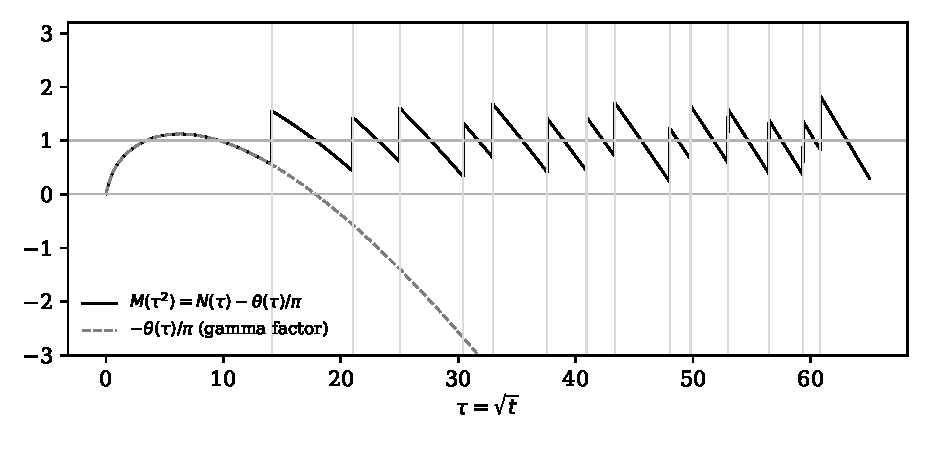
\includegraphics[width=0.9\textwidth]{rzfig/fig_M.pdf}
\caption{The function $M(\tau^2)=N(\tau)-\theta(\tau)/\pi=1+S(\tau)$ against $\tau=\sqrt t$, with the zero ordinates marked; under RH it is the distribution function of the Thorin measure of $\varphi$. The dashed curve is the gamma factor contribution $-\theta(\tau)/\pi$ alone. The function $M$ rises on $(0,\tau_0)$; beyond $\tau_0$, and so between consecutive ordinates, it decreases with slope $-\theta'(\tau)/\pi$, and at each ordinate it jumps by one. The mean level is $1$.}
\label{rz:fig:M}
\end{figure}

\subsection{L\'evy density, theta functions and a criterion for RH}\label{rz:sec:levy}

Under RH, integrating by parts in Theorem~\ref{rz:thm:thorin} and using $s/(s+t)=\int_0^\infty(1-e^{-sx})te^{-tx}dx$ turns the Thorin type representation of $\varphi$ into a L\'evy Khintchine one,
\begin{gather*}
\log\varphi(s)=-\int_0^\infty\bigl(1-e^{-sx}\bigr)\frac{w(x)}{x}\,dx,\\
w(x)=\int e^{-tx}\,dM(t),\qquad \frac{w(x)}{x}=\int_0^\infty e^{-tx}M(t)\,dt .
\end{gather*}
The function $w$, unlike $M$, can be written down without the zeros, and without RH.

\begin{theorem}\label{rz:thm:w}
Define, unconditionally,
\[
w(x)=e^{x/4}-P(x),\qquad P(x)=\frac{1}{\sqrt{4\pi x}}\sum_{n\ge2}\frac{\Lambda(n)}{\sqrt n}\,e^{-(\log n)^2/4x},\qquad x>0.
\]
Then $-\varphi'/\varphi(s)=\int_0^\infty e^{-sx}w(x)\,dx$ for $s>\frac14$, and for every $x>0$
\begin{equation}\label{rz:eq:weil}
\begin{gathered}
w(x)=W(x)-W_0(x),\qquad W(x)=\tfrac12\sum_\rho e^{x(\rho-\frac12)^2},\\
W_0(x)=\frac1\pi\int_0^\infty e^{-x\tau^2}\theta'(\tau)\,d\tau,
\end{gathered}
\end{equation}
the sum running over all nontrivial zeros with multiplicity. Here $W$ is the heat trace of Section~\ref{ch:clock} in the variable $x$; under RH, $W(x)=\sum_{\gamma>0}e^{-x\gamma^2}$ and $w(x)=\int e^{-tx}dM(t)$. The function $w$ satisfies $w(0^+)=1$ and $w(x)\sim c/(2\sqrt{\pi x})$ as $x\to\infty$.
\end{theorem}

\begin{proof}
By logarithmic differentiation, $-\varphi'/\varphi=\frac{1}{s-1/4}+\frac{1}{2\sqs}\frac{\zeta'}{\zeta}(\frac12+\sqs)$. The first term is the transform of $e^{x/4}$; for the second use $\zeta'/\zeta=-\sum\Lambda(n)n^{-z}$ and $\frac{1}{2\sqs}e^{-a\sqs}=\int_0^\infty e^{-sx}(4\pi x)^{-1/2}e^{-a^2/4x}dx$, with Tonelli justified on $s>\frac14$. Identity \eqref{rz:eq:weil} is Weil's explicit formula for the even test function $h(r)=e^{-xr^2}$, whose Fourier partner is $g(u)=(4\pi x)^{-1/2}e^{-u^2/4x}$: the pole contributes $h(\pm\frac i2)=e^{x/4}$, the archimedean place contributes $W_0$, and the primes contribute $P$. It is \eqref{eq:ch2:Warith} of Section~\ref{ch:clock} with $t=x$. Under RH, Theorem~\ref{rz:thm:thorin} gives the same Laplace transform for $\int e^{-tx}dM(t)$ and uniqueness identifies the two. The limit $w(0^+)=1$ holds because $P(x)=O(x^{-1/2}e^{-(\log2)^2/4x})$ as $x\to0$. The behaviour at infinity needs no hypothesis: every term of $W$ has modulus at most $e^{-x(\gamma^2-1/4)}$ with $\gamma>14$, so $W$ decays exponentially, while $W_0(x)\sim-c/(2\sqrt{\pi x})$ by Lemma~\ref{rz:lem:W0} below.
\end{proof}

We call $w$ the canonical function of $\varphi$: when $\varphi$ is infinitely divisible, $w(x)/x$ is its L\'evy density, and $\varphi$ is infinitely divisible exactly when $w\ge0$. Theorem~\ref{rz:thm:w} gives $w$ two faces. On the prime side $w$ is the heat trace $e^{x/4}=h(\pm\frac i2)$ of the pole, the Gaussian evaluated at the imaginary ordinate of $z=1$, minus the heat trace $P$ of the prime powers, each a Gaussian in $\log n$ of variance $2x$; this series converges absolutely for every $x>0$, which is the reason for working with the heat kernel $e^{-tx}$. On the zero side $w$ is the heat trace over the zeros minus that of their smooth count $\theta/\pi$, which comes from the gamma factor. The proof of Theorem~\ref{rz:thm:id} uses both faces, the prime side for small $x$ and the finitely many verified zeros for large $x$, and it rests on the following integral formula for $W_0$.

\begin{lemma}\label{rz:lem:W0}
For $x>0$,
\[
W_0(x)=\frac{F(x)}{4\sqrt{\pi x}},\qquad F(x)=2\theta'(0)+\int_0^\infty\frac{e^{-u/4}\bigl(1-e^{-u^2/16x}\bigr)}{1-e^{-u}}\,du .
\]
The function $F$ is strictly decreasing, $F(0^+)=+\infty$ and $F(\infty)=2\theta'(0)=\psi(\frac14)-\log\pi<0$. Hence $W_0$ has exactly one zero $x_*$, with $W_0>0$ on $(0,x_*)$ and $W_0<0$ on $(x_*,\infty)$.
\end{lemma}

\begin{proof}
Insert $\psi(z)=\int_0^\infty\bigl(e^{-u}/u-e^{-zu}/(1-e^{-u})\bigr)du$ with $z=\frac14+\frac{i\tau}2$ into $\theta'$, and use $\int_0^\infty e^{-x\tau^2}\cos(\tau u/2)\,d\tau=\frac12\sqrt{\pi/x}\,e^{-u^2/16x}$; the interchange is justified after writing the $\psi$ integrand as $e^{-u}/u-e^{-u/4}/(1-e^{-u})$ plus $e^{-u/4}(1-\cos(\tau u/2))/(1-e^{-u})$, both absolutely integrable against $e^{-x\tau^2}$. The terms free of $\tau$ reassemble into $\psi(\frac14)-\log\pi$. The integrand of $F$ is positive and decreasing in $x$; as $x\to0$ it increases to $e^{-u/4}/(1-e^{-u})$, which is not integrable at $0$.
\end{proof}

The Vere-Jones representation of Theorem~\ref{rz:thm:saw} writes $w$ as an absolutely convergent series of theta functions, one for each block. For the sawtooth measure of Lemma~\ref{rz:lem:saw} define its heat trace
\[
h_\lambda(x)=-\int e^{-tx}\,U_\lambda(dt)=\sum_{k\ge0}e^{-x\sigma_k(\lambda)}-\frac{\lambda}{4\sqrt{\pi x}}
=\frac{\lambda}{2\sqrt{\pi x}}\sum_{j\ge1}(-1)^je^{-j^2\lambda^2/4x},
\]
the last form by Poisson summation. The first form is a sum over the pseudo zeros minus their smooth count and the second a sum over the multiples $j\lambda$, so this Jacobi theta identity is the explicit formula of the toy zeta function $1+e^{-\lambda\sqs}$.

\begin{proposition}\label{rz:prop:theta}
For every $x>0$, with absolutely convergent sums,
\[
w(x)=e^{x/4}+\sum_{N\ge2}B_N\,h_{\log N}(x).
\]
\end{proposition}

\begin{proof}
Substitute the theta form of $h_\lambda$ and regroup the triple sum over $(n,m,j)$ by $r=mj$. The coefficient of $e^{-r^2(\log n)^2/4x}$ is
\[
-(4\pi x)^{-1/2}a_n\log n\sum_{mj=r}m\,d_m(-1)^{j+1},
\]
and the inner sum is $\delta_{r,1}$ because its Dirichlet series is $\eta(v)^{-1}\cdot\eta(v)$. Since $a_n\log n=\Lambda(n)/\sqrt n$ the sum equals $-P(x)$. The bound $|m\,d_m|\le m$ against Gaussian decay gives absolute convergence.
\end{proof}

Proposition~\ref{rz:prop:theta} is the Vere-Jones form of Theorem~\ref{rz:thm:w}. Unconditionally, $w$ is the Laplace transform, term by term, of the formal series $\delta_{-1/4}+\sum_NB_N\{\sum_k\delta_{\sigma_k(\log N)}-\frac{\log N}{4\pi\sqrt t}dt\}$ of sech atom lattices, with all the arithmetic in the weights $B_N$; under RH it is also the Laplace transform of $dM$. The atom at $-\frac14$ comes from the pole of $\zeta$ and lies outside $(0,\infty)$, where Thorin measures live, so under RH the sawtooth series must cancel it. Two consequences follow. The first makes the sawtooth expansion of $S$ rigorous after Gaussian averaging.

\begin{corollary}\label{rz:cor:Ssaw}
Assume RH. For every $x>0$,
\[
\int_0^\infty S(\tau)\,2\tau e^{-x\tau^2}\,d\tau=\frac{e^{x/4}-1}{x}+\sum_{N\ge2}B_N\int_0^\infty\Sigma_{\log N}(\tau)\,2\tau e^{-x\tau^2}\,d\tau,
\]
and each integral on the right equals $h_{\log N}(x)/x$.
\end{corollary}

\begin{proof}
By Theorem~\ref{rz:thm:w},
\[
\int_0^\infty e^{-tx}(1+S(\sqrt t))dt=w(x)/x,
\]
and $\int_0^\infty e^{-tx}\Sigma_\lambda(\sqrt t)\,dt=h_\lambda(x)/x$ by parts since $\Sigma_\lambda(0)=0$. Subtract $\int e^{-tx}dt=1/x$ and apply Proposition~\ref{rz:prop:theta}; substitute $t=\tau^2$.
\end{proof}

This is the sawtooth analogue of the classical formal series $S(\tau)=-\pi^{-1}\sum_na_n\sin(\tau\log n)$, with the pole appearing as the correction $(e^{x/4}-1)/x$. The second consequence is a criterion for RH.

\begin{theorem}\label{rz:thm:crit}
The following are equivalent.
\begin{enumerate}
\item[(i)] The Riemann Hypothesis.
\item[(ii)] There is a real signed Borel measure $m$ on $[0,\infty)$ with $\int|m|(dt)/(1+t)<\infty$ and $w(x)=\int e^{-tx}m(dt)$ for all $x>0$.
\end{enumerate}
In that case $m=dM$.
\end{theorem}

\begin{proof}
If RH holds take $m=dM$; the atoms satisfy $\sum(1+\gamma^2)^{-1}<\infty$ and the density is $O(t^{-1/2}(1+t)^{-1}\log(2+t))$ after division by $1+t$. Conversely, given $m$, put $J(s)=\int m(dt)/(s+t)$, analytic on $\cut$. For $s>\frac14$ Fubini gives $\int_0^\infty e^{-sx}w(x)dx=J(s)$, so $-\varphi'/\varphi=J$ on $(\frac14,\infty)$ and hence on all of $\cut$ by analytic continuation. A zero or pole of $\varphi$ in $\cut$ would be a pole of $-\varphi'/\varphi$, so $\varphi$ has none, and Proposition~\ref{rz:prop:rh} gives RH. Uniqueness of the Stieltjes transform gives $m=dM$.
\end{proof}

The criterion is a statement about $w$ alone, which is computable from the primes. In the language of Proposition~\ref{rz:prop:theta}, RH says that the formal measure $\delta_{-1/4}+\sum_NB_N(-U_{\log N})$ has the Laplace transform of a genuine real measure on $[0,\infty)$. If RH fails, a zero $\rho=\frac12+\beta+i\gamma$ with $\beta>0$ and its conjugate contribute to $W$ the term $e^{x(\beta^2-\gamma^2)}\cos(2\beta\gamma x)$, and the quadruple $\rho,\bar\rho,1-\rho,1-\bar\rho$ contributes twice this. The term is the real part of the Laplace transform of an atom at the complex point $(\gamma-i\beta)^2$, and no real measure on $[0,\infty)$ can reproduce it.

\subsection{Across the critical strip}\label{rz:sec:strip}

Moving the line of evaluation across the critical strip puts the results of this section and of Section~\ref{ch:rz3} in one picture. Fix $\sigma$ and evaluate $\zeta$ on the line $\Re z=\sigma$ through $z=\sigma+\sqs$. A zero $\rho=\beta+i\gamma$ then sits at $s=(\rho-\sigma)^2$: if $\beta>\sigma$ it gives a pole of $1/\zeta(\sigma+\sqs)$ in $\cut$, if $\beta=\sigma$ a point of the cut, and if $\beta<\sigma$ no singularity, only a Poisson kernel of width $\sigma-\beta$ in the Thorin density. On each line one can ask whether a normalised reciprocal of $\zeta$ is infinitely divisible, that is, has a L\'evy representation with positive L\'evy measure, and whether the completed function $R_\sigma(s)=\xi(\sigma)/\xi(\sigma+\sqs)$ has the stronger GGC property.

To the right of $\Re z=1$ the first question has a classical answer, in the variable $\tau$ rather than $s$. The Dirichlet series converges, $\zeta(\sigma+i\tau)/\zeta(\sigma)=\E e^{-i\tau\log N_\sigma}$ for the zeta distribution $\Pr(N_\sigma=n)=n^{-\sigma}/\zeta(\sigma)$, and the L\'evy measure of $\log N_\sigma$ is the prime measure $\sum_n\Lambda(n)n^{-\sigma}(\log n)^{-1}\delta_{\log n}$. The Vere-Jones representation writes this measure as a superposition of the alternating lattices $\sum_j(-1)^{j+1}j^{-1}\delta_{jn\log p}$, the signed L\'evy measures of fair coins, one for each prime power $p^n$, with weight the necklace polynomial $b_n(p^{-\sigma})$ (Theorem~\ref{rz:thm:necklace}). At $\sigma=0$ the weight $b_n(1)$ is $1$ when $n$ is a power of $2$ and $0$ otherwise, and the identity becomes Euler's binary product, with every block a solved model of unit multiplicity; for $\sigma>0$ the weights are fractional and some are negative.

Inside the strip $|\zeta(\sigma+i\tau)|$ is unbounded, while a characteristic function is bounded by $1$, so the characteristic function picture breaks down; the Vere-Jones representation survives in the variable $s$. For $0<\sigma<1$ put $\varphi_\sigma(s)=\zeta(\sigma)/\{(1-s/(1-\sigma)^2)\zeta(\sigma+\sqs)\}$, which is $\varphi$ at $\sigma=\frac12$. For $s>(1-\sigma)^2$, $-\varphi_\sigma'/\varphi_\sigma$ is the Laplace transform of a function $w_\sigma$, given by the theta series of Proposition~\ref{rz:prop:theta} (Section~\ref{rz:sec:levy}) with $e^{(1-\sigma)^2x}$ in place of $e^{x/4}$ and the weights $b_n(p^{-\sigma})$ in place of $B_{p^n}=b_n(p^{-1/2})$ (Theorem~\ref{rz:thm:levystrip}). When $w_\sigma\ge0$ this is a L\'evy representation, $\log\varphi_\sigma(s)=-\int(1-e^{-sx})w_\sigma(x)x^{-1}dx$, with an explicit L\'evy density built from the primes. Theorem~\ref{rz:thm:id} proves $w_{1/2}=w>0$, and numerically $w_\sigma>0$ on nine lines from $\sigma=0.05$ to $\sigma=0.99$, for $10^{-4}\le x\le10^3$ (Section~\ref{ch:rz3}); whether infinite divisibility holds on every line of the strip is open (Problem~\ref{rz:prob:strip}).

The Thorin property is where the zeros enter. The functions $\varphi_\sigma$ are never GGCs, for a reason that uses no information about $\zeta$: the factor removing the pole makes $w_\sigma$ increase at the origin (Proposition~\ref{rz:prop:onlyhalf}). For $\sigma\ge\frac12$, by Theorem~\ref{rz:thm:threshold}, the form of Theorem~\ref{thm:poisson} in the coordinates of Section~\ref{rz:sec:intro}, the function $R_\sigma$ is a GGC if and only if $\zeta(z)\ne0$ for $\Re z>\sigma$, and its Thorin measure is then the zero density smoothed by Poisson kernels of widths $\sigma-\beta$ in the variable $\sqrt t$. The smallest such $\sigma$ is $\Theta=\sup\Re\rho$, and RH is the statement $\Theta=\frac12$: the kernels then sharpen all the way to the unit atoms at $\gamma^2$ of the Thorin measure of $R$ (Proposition~\ref{prop:struct} and the paragraph after Theorem~\ref{rz:thm:threshold}). The Thorin density of the gamma factor is also built from Poisson kernels (Theorem~\ref{rz:thm:gamma}), but their widths $c_n=2n+\frac12$ are fixed and never sharpen, so the gamma factor produces no atoms. Table~\ref{rz:tab:strip} records the picture.

\begin{table}[htbp]
\centering
\small
\begin{tabular}{p{0.2\textwidth}p{0.34\textwidth}p{0.34\textwidth}}
\toprule
Line & L\'evy representation & Thorin representation of $R_\sigma$\\
\midrule
$\sigma>1$ & $\zeta(\sigma+i\tau)/\zeta(\sigma)=\E e^{-i\tau\log N_\sigma}$; prime L\'evy measure as a necklace weighted superposition of fair coin lattices & GGC, unconditionally; Thorin measure a Poisson smoothed zero density\\
$\sigma=1$ & not treated here & GGC, unconditionally; no atoms, since $\zeta$ has no zeros on $\Re z=1$\\
$\frac12<\sigma<1$ & $w_\sigma>0$ numerically & GGC if and only if there are no zeros with $\Re\rho>\sigma$\\
$\sigma=\frac12$ & $w>0$ proved & GGC if and only if RH; the Poisson kernels sharpen to atoms at $\gamma^2$\\
$\sigma<\frac12$ & $w_\sigma>0$ numerically & never: each zero on the critical line gives a pole of $R_\sigma$ in $\cut$\\
\bottomrule
\end{tabular}
\caption{The two questions across the critical strip. Middle column: the L\'evy representation, in the variable $\tau$ for $\sigma>1$ and in the heat kernel form of Theorem~\ref{rz:thm:levystrip} for $0<\sigma<1$, where the L\'evy measure is positive when $w_\sigma>0$. Right column: whether $R_\sigma$ is a GGC (Theorem~\ref{rz:thm:threshold}).}
\label{rz:tab:strip}
\end{table}

Chapters~\ref{chap:basepoint} to \ref{chap:almost} return to the completed functions $R_\sigma$, written there $\varphi_\alpha(u)=\xi(\alpha)/\xi(\alpha+\sqrt u)$, with the basepoint $\alpha$ in place of $\sigma$ and the variable $u$ of the book in place of $s$; they are not the normalised functions $\varphi_\sigma$ of this section. Section~\ref{ch:basepoint} studies the basepoint $\alpha=1$, the leftmost at which the GGC property is a theorem, Section~\ref{ch:strip} shows that $\xi(\alpha)/\xi(\alpha+|v|)$, as a function of real $v$, is the characteristic function of a normal scale mixture at every basepoint, and Section~\ref{ch:almost} shows by zero density estimates that for every $\alpha>\frac12$ the negative part of the Thorin measure up to height $T$, if there is one, is a vanishing proportion of the whole as $T\to\infty$.
